\documentclass[12pt]{article}
\usepackage{graphicx}
\usepackage{xcolor}
\usepackage{geometry}
\geometry{margin=1in}

\begin{document}

\begin{center}
\includegraphics[width=0.3\textwidth]{images/iiitb_logo.png.jpg}
\end{center}

\begin{center}
\textbf{\Large Harshita N Kumar} \\
\textbf{ID: COMETFWC052}
\end{center}

\vspace{0.5cm}

\begin{center}
{\color{blue}\Huge GATE Question No. 41}
\end{center}

\vspace{0.5cm}

{\color{blue}\Large Question}

\vspace{0.3cm}

\includegraphics[width=\textwidth]{images/question41.jpg}

\vspace{0.5cm}

{\color{blue}\Large Given Circuits}

\vspace{0.3cm}

\includegraphics[width=\textwidth]{images/gates41.jpg}

\vspace{0.5cm}

{\color{blue}\Large Question Analysis}

The problem states that three circuits produce the same output and one circuit produces a different output.

After simplifying the expressions:

Option (a), (b), and (c) reduce to:

$Q = A\overline{B}$

Option (d) reduces to:

$Q = \overline{A} + B$

Since these two expressions are different, option (d) is the incorrect one.

\vspace{0.5cm}

{\color{blue}\Large Truth Table for $Q = A\overline{B}$}

\begin{center}
\begin{tabular}{|c|c|c|}
\hline
A & B & Q \\
\hline
0 & 0 & 0 \\
0 & 1 & 0 \\
1 & 0 & 1 \\
1 & 1 & 0 \\
\hline
\end{tabular}
\end{center}

\vspace{0.5cm}

{\color{blue}\Large Hardware Implementation}

The function implemented using Arduino and 7447:

$Q = A\overline{B}$

Connections:

\begin{itemize}
\item Arduino Pin 10 $\rightarrow$ Input A
\item Arduino Pin 11 $\rightarrow$ Input B
\item Arduino Pin 9 $\rightarrow$ 7447 Pin 7
\item 7447 Pin 16 $\rightarrow$ 5V
\item 7447 Pin 8 $\rightarrow$ GND
\item 7447 Pins 3,4,5 $\rightarrow$ 5V
\item 7447 Pins 1,2,6 $\rightarrow$ GND
\item 7-segment common pins $\rightarrow$ 5V
\end{itemize}

\vspace{0.3cm}

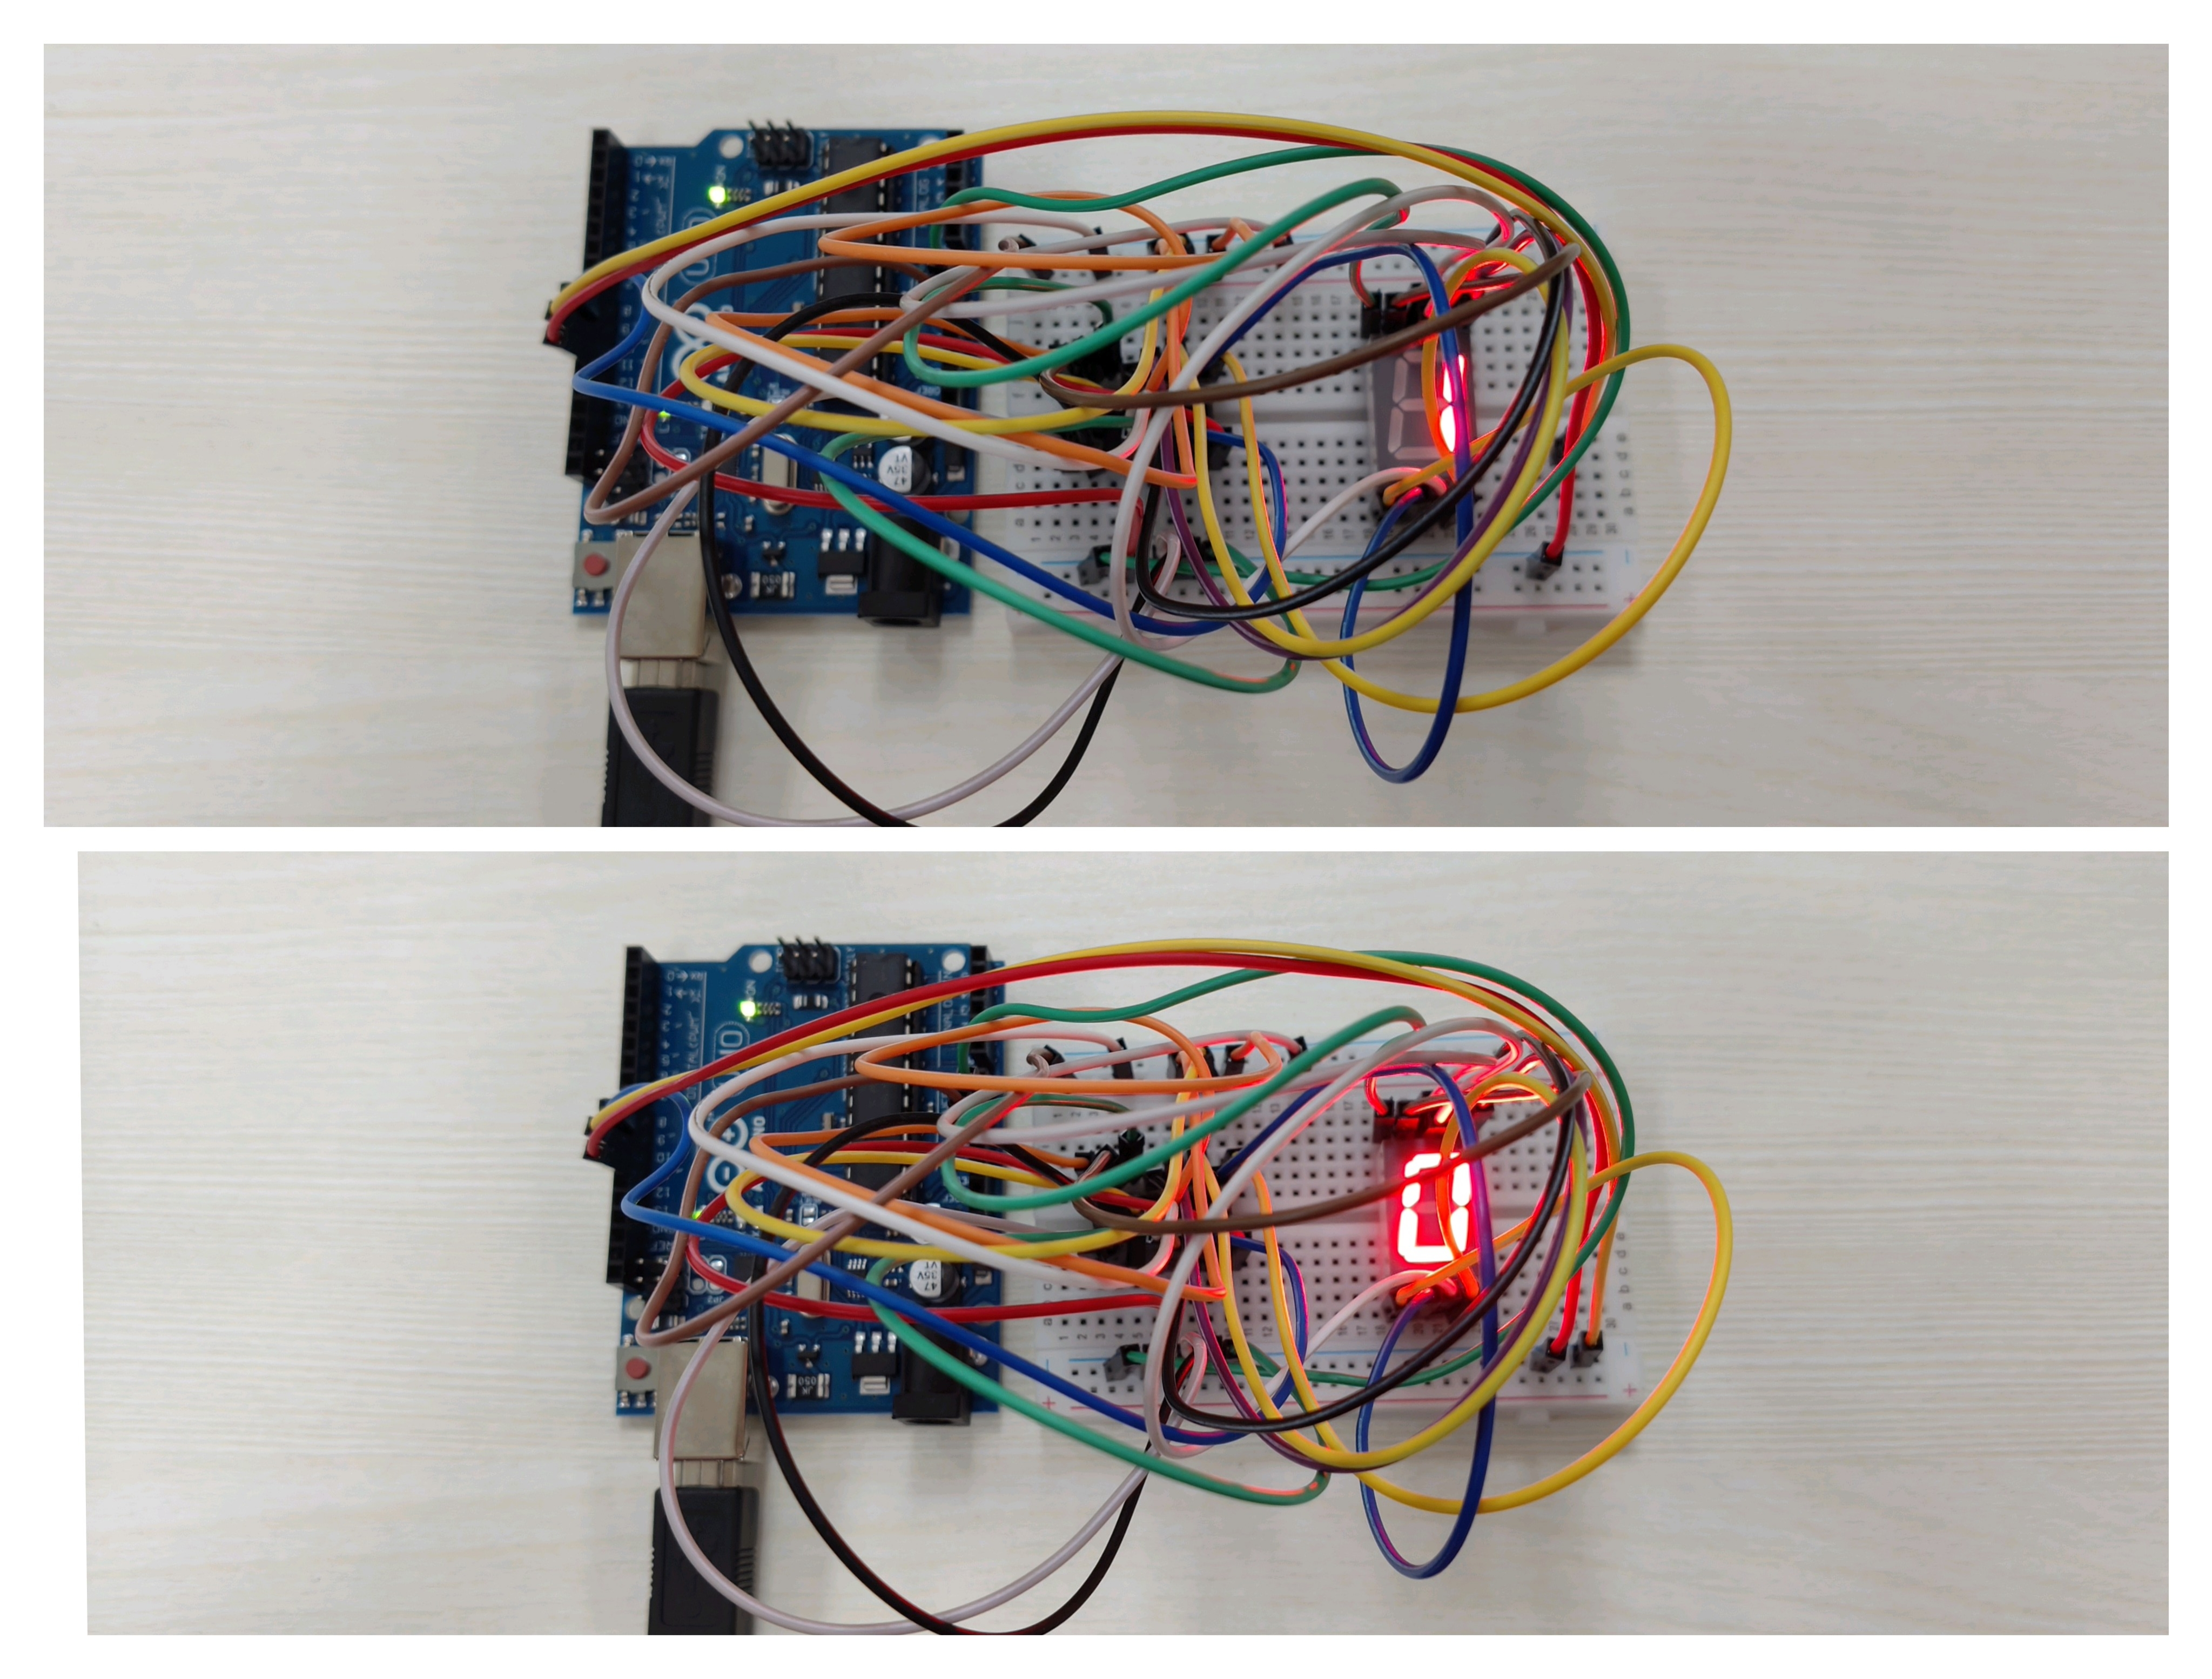
\includegraphics[width=\textwidth]{images/hardware41.jpg}

\vspace{0.5cm}

{\color{blue}\Large Code Uploading Steps}

\begin{enumerate}
\item Create a PlatformIO project.
\item Write the code in main.cpp inside src folder.
\item Run the command: \texttt{pio run}
\item Copy the generated .hex file to Arduino Droid folder.
\item Connect Arduino UNO using OTG cable.
\item Use Upload Precompiled option.
\item Observe the output on 7-segment display.
\end{enumerate}

\vspace{0.5cm}

{\color{blue}\Large Experimental Verification}

\begin{center}
\begin{tabular}{|c|c|c|}
\hline
A & B & Displayed Output \\
\hline
0 & 0 & 0 \\
0 & 1 & 0 \\
1 & 0 & 1 \\
1 & 1 & 0 \\
\hline
\end{tabular}
\end{center}

\vspace{0.5cm}

{\color{blue}\Large Conclusion}

From Boolean simplification and hardware verification, circuits (a), (b), and (c) implement $Q = A\overline{B}$.

Circuit (d) implements $Q = \overline{A} + B$.

Therefore, option (d) is the incorrect circuit.

\end{document}
